%!TEX root = ../../../main.tex
\section{Navigation} % (fold)
\label{sec:mr_navigation}
In this section the different types of navigation that let the robot move are explained.
These are the actions of the robot that let the robot change its position and they are used as means by the navigation controller (\ref{sec:mr_navigation_controller}) to move around the workplace.
As will be explained in the section \ref{sec:mr_safety_system}, this states are the only ones that activate the deadman signal that let the robot move.
These states are intrinsically exclusive, meaning that, for example, line navigation and free navigation can't be used at the same time.

    \subsection{Relative navigation} % (fold)
    \label{sub:mr_relative_navigation}
    Making use of the combined odometry from the wheels and the IMU, the relative navigation has been implemented.
    Two different movements can be carried out: angular and linear.
    While angular can rotate the robot over the rotation axis given by the position of the wheels (clockwise or anticlockwise), the linear can shift the robot in a straight line of its position (forward or backward).
    This two movements are represented in the figures \ref{fig:mr_relative_linear} and \ref{fig:mr_relative_angular} respectively.

    The relative movement is based on a P controller that tries to minimize the error between the current position and the desired position, which is calculated from the current position and the required movement.

   \begin{figure}
        \centering
        \begin{subfigure}[b]{0.25\textwidth}
            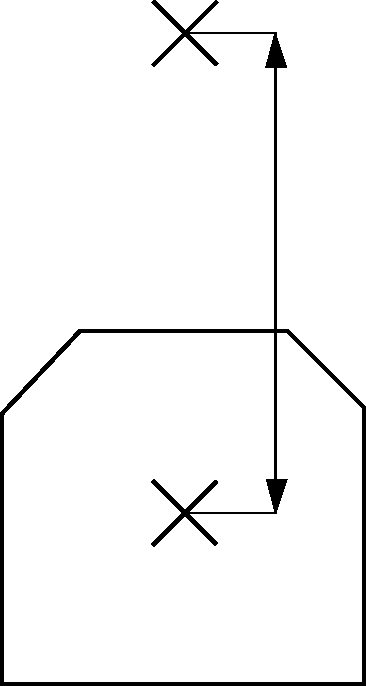
\includegraphics[width=\textwidth]{figs/mr_relative_linear}
            \caption{Linear movement representation}
            \label{fig:mr_relative_linear}
        \end{subfigure}
        \hspace{40pt}
        \begin{subfigure}[b]{0.296\textwidth}
            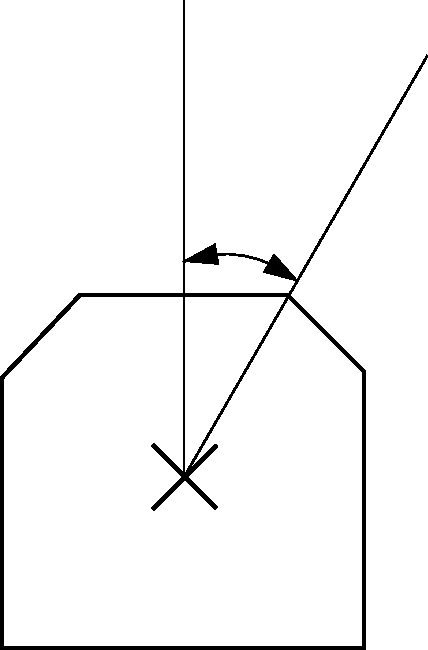
\includegraphics[width=\textwidth]{figs/mr_relative_angular}
            \caption{Angular movement representation}
            \label{fig:mr_relative_angular}
    \end{subfigure}
    \caption{Representation of the relative movements}
    \end{figure}
    % subsection relative_navigation (end)



    \subsection{Line navigation} % (fold)
    \label{sub:mr_line_navigation}
    Taking the information from the camera processing a PID is used to track the line.
    This PID tries to minimize the distance between the point that represents the center of the line and a desired point.
    The desired point is the center of the image due to the camera was physically positioned in the perpendicular to the rotation axis of the robot.
    % subsection line_navigation (end)



    \subsection{Free navigation} % (fold)
    \label{sub:mr_free_navigation}

    When the robot reaches the end of the line it needs to navigate  to and in the box containing the charging station and brick dispenser. For localisation in this area the LIDAR, odometry and a camera localization system is available. The camera system is used to initialize the particle filter used for navigation. The system requires a marker placed on the robot visible from the roof mounted  camera. This systems is currently not used on the robot. The system was discarded due to the performance of the LIDAR localisation in the area the camera system covers. The removal of the marker from the top of the mobile platform increased the area for catching dispensed bricks thus reducing the required precision for navigating to the brick dispenser. For these reasons the camera system is disabled. 
    
    As per project description, the navigation inside the box is to be done based on SLAM. 
    Due to complexity of the entire project and potential diversity of SLAM implementations, an open-source implementation of SLAM was chosen. 
    More specifically the gmapping-package \cite{gmapping} which has a livid community of supporters and builds a ROS wrapper for “OpenSlam's Gmapping”\cite{openslam}. 
	\begin{figure}[H]
        \centering
        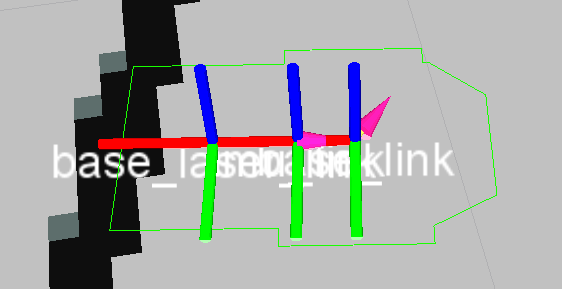
\includegraphics[width=0.5\textwidth]{mr_slam_tf}
        \caption{TF Frames}
        \label{fig:tf_frames}
    \end{figure}
    TF-Frames of LIDAR, IMU and the robot base were set up, see Figure \ref{fig:tf_frames} , this allows for easy transformation between LIDAR and odometry data, inside the package. 
    Using these, the SLAM-Implementation uses a particle filter to sequentially build up a map of the area. 
    By manually driving through the entire workspace, a map was created. 
    \begin{figure}[H]
        \centering
        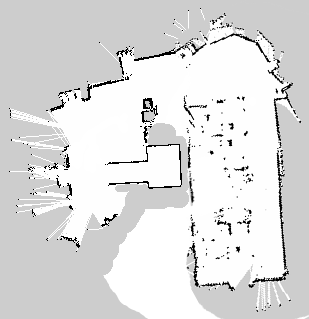
\includegraphics[width=0.5\textwidth]{slam_map}
        \caption{Slam Map}
        \label{fig:slam_map}
    \end{figure}
    Using the map-server package from the ROS 2D-Navigation Stack \cite{navigation_stack} the generated map was stored, see Figure \ref{fig:slam_map} and is then broadcasted as a static map for localization.
   \begin{figure}[H]
        \centering
        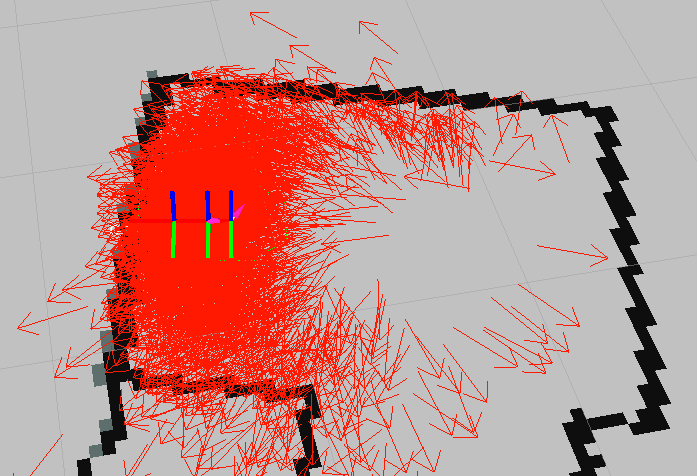
\includegraphics[width=0.5\textwidth]{mr_amcl}
        \caption{Particle Cloud}
        \label{fig:particle_cloud}
    \end{figure}
    The AMCL (Adaptive Monte-Carlo Localization) package (which is also included in the navigation stack) then uses the static map, the LIDAR as well as odometry data and a particle cloud (as seen in Figure \ref{fig:particle_cloud} to localize the robot while in free navigation. A particle  
    After tuning the parameters, AMCL worked fairly reliably for navigation both inside and outside the box.\\
	The path planning and execution used for navigating in and outside of the box is done with the ROS package move{\_}base. The package uses two path planners, a global and a local, each of these planners maintains a costmap. The costmap for the global planner contains the map of the area and in this costmap a path from the current pose to the goal pose is calculated. When the global planner succeeds in creating a path the local planner takes over. This planner generates multiple plans with the parameters linear and angular speed. These plans are evaluated based on the reduced distance to the goal, the distance to the path and distance to obstacles. \\
	In situations where the local planner is unable to complete the navigation a number of recovery behaviours is executed. Initially obstacles further away that 3 meters are cleared. If this does not prove successful the robot performs an in place rotation to clear local obstacles. This also helps the AMCL in adjusting the position of the robot which has proved particularly useful when navigating inside box. Is the navigation still failing all obstacles outside the area of the rotation are cleared. 
    \\
    Due to the box being fairly monotone in respect to the LIDAR readings (clean, walls, no landmarks), precise navigation inside the box was sometimes not perfect. 
    Also with multiple robots present in the box, issues, especially when trying to charge occurred. 
    To ensure reliability of charging a line was added, using the already implemented Line Following behaviour. 
    The move{\_}base is used to navigate the robot to the start of the charging line. 
    Then the robot follows the line until a pre-specified distance from the wall using LIDAR. 
    If the battery level is increasing, the behaviour is successful, otherwise it will try again. This proved to be reliable in successful charging.\\
    % subsection free_navigation (end)

    \subsection{Manual navigation} % (fold)
    \label{sub:mr_manual_navigation}
    The ability to control the robot manually from the HMI is also implemented.
    This controller (see Figure \ref{fig:mr_manual_navigation}) shown in the \emph{Advanced mode} of the HMI, lets the user to control the linear and angular motions as well as the speed of these.
    This behavior is only allowed when all the skills and routines of the robot have finished so the manual mode cannot overwrite the automatic plans of the robot.

    \begin{figure}[H]
        \centering
        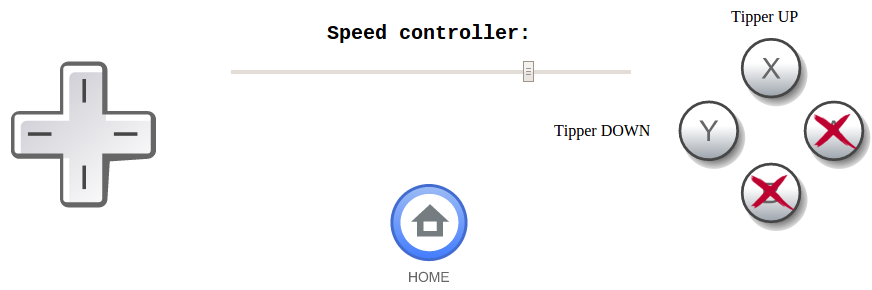
\includegraphics[width=0.7\textwidth]{figs/manual_navigation}
        \caption{Manual navigation controller in the HMI.}
        \label{fig:mr_manual_navigation}
    \end{figure}
    
    % subsection manual_navigation (end)

% section navigation (end)